\documentclass[../thesis]{subfiles}

\begin{document}

\chapter{Summary}
This thesis has provided a review of the design and implementation of
software systems for facilitating reproducible research and has
described eGor, a toolkit for collaboratively specifying, executing,
and analyzing real-world experiments. The completed design has a
number of subsystems and draws inspiration from a number of existing
free and commercial software packages, and would not be possible
without the huge range of open source libraries available for web
programming today. Nevertheless, creating eGor has involved solving a
number of difficult software development problems and has resulted in
several design approaches and capabilities that appear to be
unique. While minimum functionality has been achieved, this project is
an ongoing effort and will rely on continued contribution from core
developers and the open-source community to make a truly powerful
framework.



\section{Contributions}
eGor was designed in response to a set of challenges that are not
adequately addressed by existing scientific software. The tool
described in this thesis combines a number of features that have not
previously been explored in this application domain, centered around a
modern, flexible web application architecture built on a broad range
of advanced software technologies and design patterns. Here we
reiterate the unique features of the system and their value for
automated, reproducible research as well as other large scale web
applications.

\subsection{Hardware-connected lab informatics}
eGor represents the only software solution we are aware of for
cloud-based structured management of experimental data and procedures
that is also capable of directly interacting with arbitrary commercial
or custom hardware. The system's design allows users to remotely
control lab equipment via an ordinary browser interface, but also
allows scheduled sequences of device commands and parameters to be
captured alongside datasets, discussion, and analysis in an electronic
lab notebook document. Raw datasets and the metadata necessary for
their interpretation can be automatically recorded in a richly
structured archival format, allowing collaborators or reviewers to
examine, analyze, and share the complete lifecycle of an experiment
involving manipulations of physical equipment as well as sophisticated
software analysis. We believe that this integrated set of capabilities
will improve researcher productivity, the reproducibility of
scientific work, and the state of software-driven scientific workflows
in general.

\subsection{Modularity via microservices}
The core of eGor's design is its focus on subdividing functionality
into small functional subsystems called microservices which
communicate over ordinary network protocols and may be composed into
larger systems. This is not a design innovation on its own, and in
fact is being increasingly adopted by a number of technology companies
to power their internal operations. However, eGor makes extensive use
of dynamic module loading to allow new microservices to be created and
enabled at runtime and seamlessly integrated with existing
functionality. This behavior is made possible by a special
microservice responsible for installing other services. By
compartmentalizing each service into its own version-control
repository, ystem components can also be upgraded using this mechanism
whenever they change, allowing the entire system to cooperate with
continuous integration strategies and making sure all users stay
up-to-date. Additionally, each device driver is encapsulated in a
service, and this strategy at once simplifies the design and makes it
possible for users and eGor developers to add support for new devices
far into the future.

\subsection{Design for customizability}
The ability to dynamically load new services also provides users with
a powerful mechanism for customizing and extending the eGor system to
meet their needs. Ultimately the developers envision an ecosystem
where researchers can create and share services independently,
collaboratively extending eGor in much the same way as scientists
share publications or technical tips. eGor's design is marked by focus
on user customization, and we provide libraries for creating new
device drivers and user interface components. User interface
components may also be loaded dynamically into the browser interface,
and each service or device driver may be associated with any number of
these graphical control panels. The browser app makes use of a ``hot
reloading'' approach to allow parts of the page to be updated without
performing a complete refresh, enabling a very fast development cycle
for users to create and customize their control panels. We believe
the novel architectural choices made to enable these capabilities will
help to overcome the limited longevity of many lab informatics
software packages.



\section{Implementation status and future work}
The design vision elaborated in this thesis is ambitious and has not
yet been completely realized. At the time of this writing the system's
core architecture is in place, but some usability features have yet to
be implemented. The infrastructure for dynamically loading
microservices and communicating between them has been completed, and
the system can automatically detect connected devices, look up
appropriate drivers by querying our internal server, and bind the
driver to the connected port. Real-time remote interaction with
devices via the browser interface is available, as shown in Figure
\ref{fig:browser-interface}. A small set of device drivers for the
equipment used by our collaborators has been implemented by composing
together simple protocol and control elements from a library provided
as part of the eGor system.

\begin{figure}
  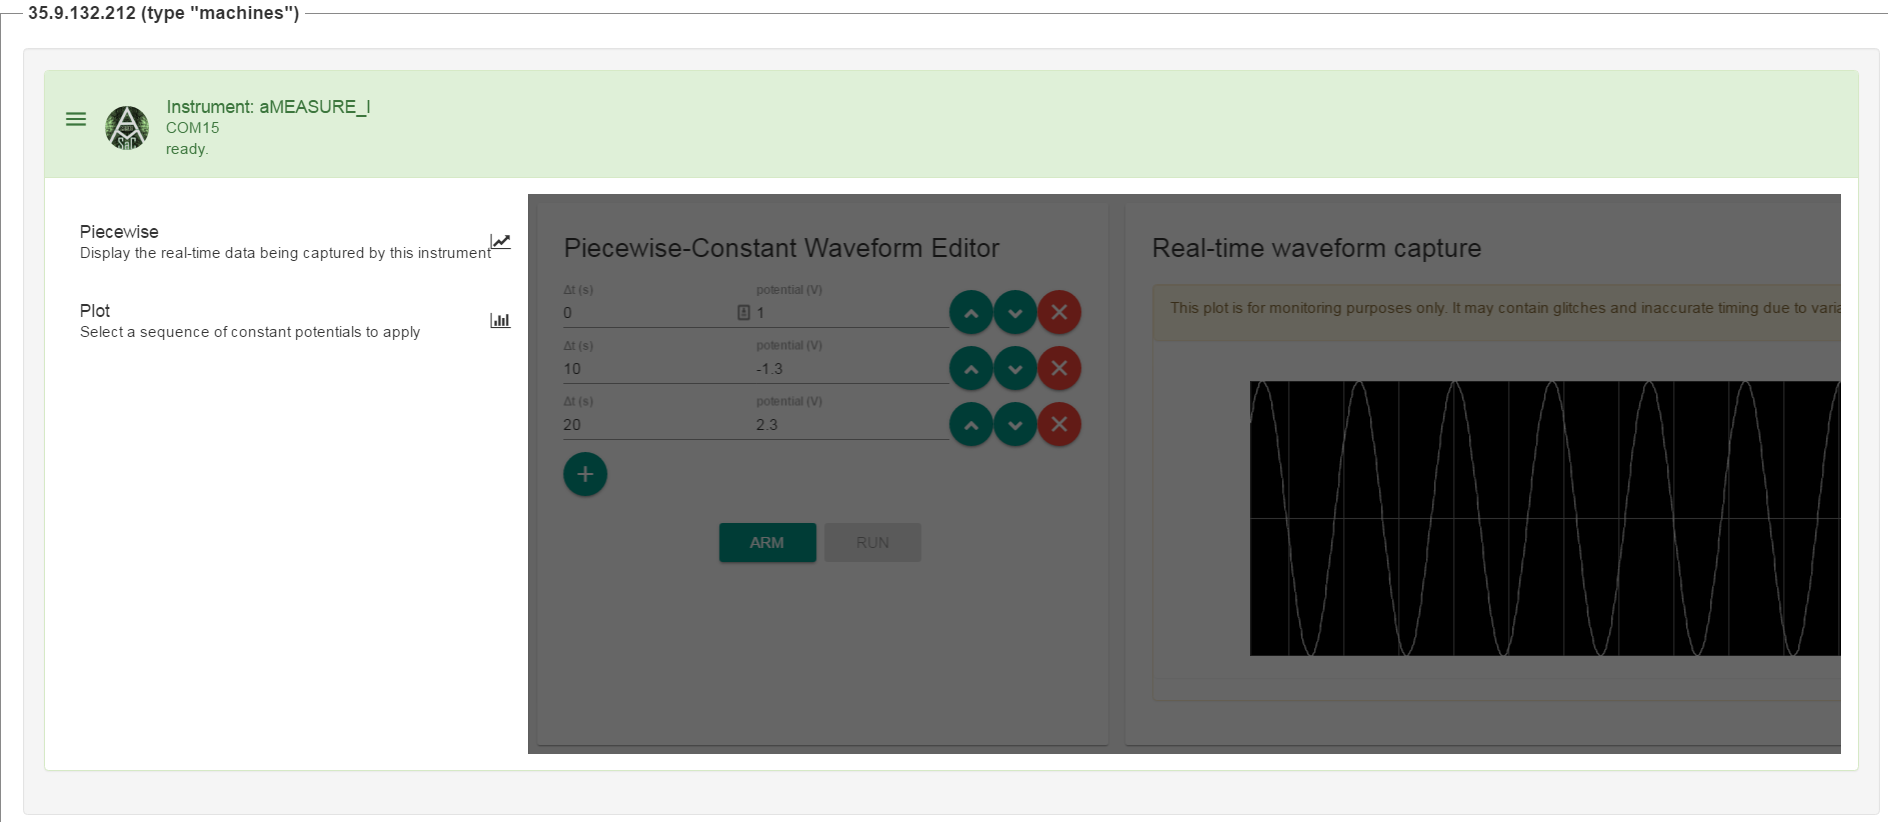
\includegraphics[width=\textwidth]{images/control-panels}
  \caption{
    Screenshot from the web browser front-end, showing a user
    interacting with a remote piece of equipment. Data may be captured
    and monitored in real time, and the device may be controlled
    either using graphical interface elements or directly
    communicating with the device over a browser-embedded terminal.
    \label{fig:browser-interface}
  }
\end{figure}

An archiving subsystem has also been developed, allowing data streams
from multiple devices to be permanently recorded in an efficiently
indexable table format. These data tables are cross-referenced with a
database of user-provided metadata describing the experiment which
created them, and can be examined via the user interface and
downloaded for external use. This functionality is intended to allow
researchers to manage their datasets alongside the specifications for
their experiments, ultimately building publication units which include
detailed links to all the research artifacts that contributed to a set
of findings.

Given the scope of eGor's application domain and the opportunities
such a tool provides for researcher productivity and scientific
auditability, the developers have begun to maintain large and
continually growing list of desired features. Much of the
functionality still to be implemented has to do with improving the
richness of the experiment metadata model. In particular, researchers
should be able to compare different experimental trials and
configurations to better understand the impact of changing a parameter
or piece of equipment. A more object-oriented approach for defining
and refining experiment templates would also be beneficial for
improving research productivity, and an object database may be a good
fit for improving how systems are modeled. Additionally, given the
infrastructure already in place it should be straightforward to expand
the existing system to allow interaction between many different
machines and independent eGor installations, but this functionality
was not necessary to our immediate use case and is not yet
implemented.



\section{Conclusion}
As it exists, eGor is usable for remotely controlling devices and for
capturing and sharing data in richer formats than are currently
typically found in ad-hoc scientific data collection. The core
architecture has been implemented for allowing user interface
components, database access layers, and device drivers to interact,
and due to the architectural focus on modularity and runtime
extensibility we believe that future users will be able to gradually
extend the system to meet their unique research goals. The current
implementation acts as a usable proof of concept for the vision
elaborated in this thesis, connecting researchers, equipment,
and data in unprecedented ways using the nascent Internet of Things as
a technological substrate.



\end{document}
